%% This is the ctufit-thesis example file. It is used to produce theses
%% for submission to Czech Technical University, Faculty of Information Technology.
%%
%% Get the newest version from
%% https://gitlab.fit.cvut.cz/theses-templates/FITthesis-LaTeX
%%
%%
%% Copyright 2021, Eliska Sestakova and Ondrej Guth
%%
%% This work may be distributed and/or modified under the
%% conditions of the LaTeX Project Public Licenese, either version 1.3
%% of this license or (at your option) any later version.
%% The latest version of this license is in
%%  https://www.latex-project.org/lppl.txt
%% and version 1.3 or later is part of all distributions of LaTeX
%% version 2005/12/01 or later.
%%
%% This work has the LPPL maintenance status `maintained'.
%%
%% The current maintainer of this work is Ondrej Guth.
%% Contact ondrej.guth@fit.cvut.cz for bug reports.
%% Alternatively, submit bug reports into the tracker at
%% https://gitlab.fit.cvut.cz/theses-templates/FITthesis-LaTeX/issues
%%
%%

%%%%%%%%%%%%%%%%%%%%%%%%%%%%%%%%%%%%%%%%%
% CLASS OPTIONS
% language: czech/english/slovak
% thesis type: bachelor/master/dissertation
%%%%%%%%%%%%%%%%%%%%%%%%%%%%%%%%%%%%%%%%%
\documentclass[czech,master,unicode]{ctufit-thesis}

%%%%%%%%%%%%%%%%%%%%%%%%%%%%%%%%%%
% FILL IN THIS INFORMATION
%%%%%%%%%%%%%%%%%%%%%%%%%%%%%%%%%%
\ctufittitle{Analýza nálady v komunikačních aplikacích} % replace with the title of your thesis
\ctufitauthorfull{Bc. Tomáš Valenta} % replace with your full name (first name(s) and then family name(s) / surname(s)) including academic degrees
\ctufitauthorsurnames{Valenta} % replace with your surname(s) / family name(s)
\ctufitauthorgivennames{Tomáš} % replace with your first name(s) / given name(s)
\ctufitsupervisor{Ing. Pavel Švagr} % replace with name of your supervisor/advisor (include academic degrees)
\ctufitdepartment{Katedra aplikované matematiky} % replace with the department of your defence
\ctufityear{2023} % replace with the year of your defence
\ctufitdeclarationplace{Praze} % replace with the place where you sign the declaration
\ctufitdeclarationdate{\today} % replace with the date of signature of the declaration
\ctufitabstractCZE{TODO CZE abstract.}
\ctufitabstractENG{TODO ENG abstract.}
\ctufitkeywordsCZE{TODO, list, of, keywords, in, CZECH}
\ctufitkeywordsENG{TODO, list, of, keywords, in, ENGLISH}
%%%%%%%%%%%%%%%%%%%%%%%%%%%%%%%%%%
% END FILL IN
%%%%%%%%%%%%%%%%%%%%%%%%%%%%%%%%%%

%%%%%%%%%%%%%%%%%%%%%%%%%%%%%%%%%%
% CUSTOMIZATION of this template
% Skip this part or alter it if you know what you are doing.
%%%%%%%%%%%%%%%%%%%%%%%%%%%%%%%%%%

\RequirePackage{iftex}[2020/03/06]
\iftutex % XeLaTeX and LuaLaTeX
    \RequirePackage{ellipsis}[2020/05/22] %ellipsis workaround for XeLaTeX
\else
    \RequirePackage[utf8]{inputenc}[2018/08/11] %this file encoding
    \RequirePackage{lmodern}[2009/10/30] % vector flavor of Computer Modern font
\fi

% hyperlinks
\RequirePackage[pdfpagelayout=TwoPageRight,colorlinks=false,allcolors=decoration,pdfborder={0 0 0.1}]{hyperref}[2020-05-15]

% uncomment the following to hide all hyperlinks
% \RequirePackage[pdfpagelayout=TwoPageRight,hidelinks]{hyperref}[2020-05-15]

\RequirePackage{pdfpages}[2020/01/28]

\setcounter{secnumdepth}{4} % numbering sections; 4: subsubsection



%%%%%%%%%%%%%%%%%%%%%%%%%%%%%%%%%%
% CUSTOMIZATION of this template END
%%%%%%%%%%%%%%%%%%%%%%%%%%%%%%%%%%


%%%%%%%%%%%%%%%%%%%%%%
% DEMO CONTENTS SETTINGS
% You may choose to modify this part.
%%%%%%%%%%%%%%%%%%%%%%
\usepackage{dirtree}
\usepackage{lipsum,tikz}
\usepackage[czech,ruled,noline]{algorithm2e}
\usepackage{csquotes}
\usepackage[style=iso-numeric]{biblatex}
\addbibresource{text/bib-database.bib}
\usepackage{listings} % typesetting of sources
% \usepackage{minted} % typesetting of sources

\usepackage{xcolor} 
\newcommand{\todo}[1]{\textcolor{red}{\textbf{[[#1]]}}}

\usepackage{blindtext}
\newcommand{\blind}[1][1]{\textcolor{gray}{\Blindtext[#1][1]}}

%theorems, definitions, etc.
\theoremstyle{plain}
\newtheorem{theorem}{Věta}
\newtheorem{lemma}[theorem]{Tvrzení}
\newtheorem{corollary}[theorem]{Důsledek}
\newtheorem{proposition}[theorem]{Návrh}
\newtheorem{definition}[theorem]{Definice}
\theoremstyle{definition}
\newtheorem{example}[theorem]{Příklad}
\theoremstyle{remark}
\newtheorem{note}[theorem]{Poznámka}
\newtheorem*{note*}{Poznámka}
\newtheorem{remark}[theorem]{Pozorování}
\newtheorem*{remark*}{Pozorování}
\numberwithin{theorem}{chapter}
%theorems, definitions, etc. END
%%%%%%%%%%%%%%%%%%%%%%
% DEMO CONTENTS SETTINGS END
%%%%%%%%%%%%%%%%%%%%%%

\begin{document} 
\frontmatter\frontmatterinit % do not remove these two commands

\includepdf{valent13-assignment.pdf} % replace that file with your thesis assignment provided by study office

\thispagestyle{empty}\cleardoublepage\maketitle % do not remove these three commands

\imprintpage % do not remove this command

\tableofcontents % do not remove this command
%%%%%%%%%%%%%%%%%%%%%%
% list of other contents: figures, tables, code listings, algorithms, etc.
% add/remove commands accordingly
%%%%%%%%%%%%%%%%%%%%%%
\listoffigures % list of figures
\begingroup
\let\clearpage\relax
\listoftables % list of tables
\lstlistoflistings % list of source code listings generated by the listings package
% \listoflistings % list of source code listings generated by the minted package
\endgroup
%%%%%%%%%%%%%%%%%%%%%%
% list of other contents END
%%%%%%%%%%%%%%%%%%%%%%

%%%%%%%%%%%%%%%%%%%
% ACKNOWLEDGMENT
% FILL IN / MODIFY
% This is a place to thank people for helping you. It is common to thank your supervisor.
%%%%%%%%%%%%%%%%%%%
\begin{acknowledgmentpage}
	Chtěl bych poděkovat především TODO
\end{acknowledgmentpage} 
%%%%%%%%%%%%%%%%%%%
% ACKNOWLEDGMENT END
%%%%%%%%%%%%%%%%%%%


%%%%%%%%%%%%%%%%%%%
% DECLARATION
% FILL IN / MODIFY
%%%%%%%%%%%%%%%%%%%
% INSTRUCTIONS
% ENG: choose one of approved texts of the declaration. DO NOT CREATE YOUR OWN. Find the approved texts at https://courses.fit.cvut.cz/SFE/download/index.html#_documents (document Declaration for FT in English)
% CZE/SLO: Vyberte jedno z fakultou schvalenych prohlaseni. NEVKLADEJTE VLASTNI TEXT. Schvalena prohlaseni najdete zde: https://courses.fit.cvut.cz/SZZ/dokumenty/index.html#_dokumenty (prohlášení do ZP)
\begin{declarationpage}
\todo{FILL IN ACCORDING TO THE INSTRUCTIONS. VYPLŇTE V SOULADU S POKYNY.}
\end{declarationpage}
%%%%%%%%%%%%%%%%%%%
% DECLARATION END
%%%%%%%%%%%%%%%%%%%

\printabstractpage % do not remove this command

%%%%%%%%%%%%%%%%%%%
% SUMMARY
% FILL IN / MODIFY
% OR REMOVE ENTIRELY (upon agreement with your supervisor)
% (appropriate to remove in most theses)
%\begin{summarypage}
%\section*{Summary section}
%\lipsum[1][1-8]
%\section*{Summary section}
%\lipsum[2][1-6]
%\section*{Summary section}
%\lipsum[3]
%\section*{Summary section}
%\lipsum[2]
%\section*{Summary section}
%\lipsum[1][1-8] Lorem lorem lorem.
%\end{summarypage}
% SUMMARY END
%%%%%%%%%%%%%%%%%%%

%%%%%%%%%%%%%%%%%%%
% ABBREVIATIONS
% FILL IN / MODIFY
% OR REMOVE ENTIRELY
% List the abbreviations in lexicography order.
%%%%%%%%%%%%%%%%%%%
\chapter{Seznam zkratek}
	
\begin{tabular}{rl}
TODO & \todo{Dodělat seznam zkratek}\\
\end{tabular}
%%%%%%%%%%%%%%%%%%%
% ABBREVIATIONS END
%%%%%%%%%%%%%%%%%%%

\mainmatter\mainmatterinit % do not remove these two commands

%%%%%%%%%%%%%%%%%%%
% THE THESIS
% MODIFY ANYTHING BELOW THIS LINE
%%%%%%%%%%%%%%%%%%%
% Kapitola Uvod
\chapter*{Úvod}\addcontentsline{toc}{chapter}{Introduction}\markboth{Introduction}{Introduction}
\setcounter{page}{1}

\todo{Napsat uvod}
\blind[4]
\subsection*{Cíle práce}
\todo{Napsat cíle práce}
\blind[2]
 % include `text.tex' from `text/' subdirectory

% Kapitola Teorie
\chapter{Teoretická východiska práce}

\begin{chapterabstract}
	V této kapitole se budeme zabývat teoretickými východisky práce a vymezením používaných pojmů.
	 Také si ukážeme existující řešení problémů podobných našemu.
	 TODO Doplnit abstract Teorie
\end{chapterabstract}

\section{Analýza sentimentu}
Na poli výzkumu dolování dat z textu můžeme narazit na dva pojmy, které jsou zaměnitelné. Jedná se o \textit{Analýzu sentimentu (SA)} a \textit{Opinion mining (OM)}. \cite{Medhat} Někteří autoři je ale rozlišují. Například Tsytsarau a Palpanas uvádějí \cite{survey}, že OM extahuje a analyzuje názor lidí vázající se k nějakému objektu či entitě, kdežto SA pouze identifikuje sentiment vyjádřený v textu a ten pak analyzuje. \marginpar{\todo{pozn. redakce: Víc mi teda sedí to vyjádření že SA a OM jsou jiné, ale uvidim}}
Podle Medhata a spol. můžeme SA rozdělit na 3 klasifikační úrovně \cite{Medhat}:
\begin{description}
	\item[Document-level] Základní jednotkou informace je jeden dokument (týkající se jednoho tématu)

	\item[Sentence-level] Určuje sentiment na základě jedné věty. 
	
	\item[Aspect-based] Určuje sentiment s ohledem na entity a jejich aspekty, kde autoři názoru mohou poskytovat různé názory na různé aspekty jedné entity (např. \uv{V této firmě se necítím dobře, ale platové podmínky jsou nejlepší na trhu}).
\end{description}

Feldman k těmto úrovním přidává ještě další 2 \cite{Feldman}:
\begin{description}
	\item[Komparativní] Základní jednotkou informace je jeden dokument (týkající se jednoho tématu)
	
	\item[Lexicon acquisition] Určuje sentiment na základě jedné věty. Není nijak zvláště rozdílná od Dokument-level analýzy, protože věty jsou v principu jen krátké dokumenty. 
	
\end{description}

\subsection{Document-level}
Jedná se o nejjedodušší formu SA. Jak již bylo řečeno, základní jednotkou informace této metody je jeden dokument a předpokládá se, že zde autor vyjadřuje svůj názor na jeden objekt. Existují dva hlavní přístupy řešení a to: supervizované a nesupervizované učení. Supervizované učení v tomto případě předpokládá, že existuje konečná množina tříd, reprezentující hledaný sentiment.  V nejjedodušším případě si vystačíme s 2 třídama, konkrétně negativní a pozitivní sentiment. Obecně se tak jedná o nějakou diskrétní škálu hodnot. 
Nesupervizované učení využívá Semantic orientation (dále jen SO) \todo{SO = kapitola?} konkrétních slov nebo vět. 
\subsection{Sentence-level}
Pokud problém vyžaduje detailnější analýzu, než poskytuje Document-level, využijeme Sentence-level metodu. Prvotně musíme věty rozdělit na subjektivní a objektivní. Objektivní věty se pro další analýzu často nevyužívají, ale některé přístupy využívají oba typy vět. Po rozdělení můžeme opět využít buďto supervizované nebo nesupervizované učení, stejně tak jako u Dokument-level analýzy.
Narayanan a spol. ukázali, že je vhodné na různé věty používat různé metody \cite{Feldman24}. Konrétně věty různých typů: tázací, podmiňovací a sarkastické. 
\subsection{Aspect-level}
Předchozí 2 typy byly předpokládaly že se každý dokument nebo věta váže k jednomu objektu. V mnoha případech však lidé hovoří o více objektech s více aspekty (objektem může být např. mobilní telefon, u kterého se můžeme vyjádřit k jeho aspektům (rychlost, velikost, paměť, atd.) kladně i záporně). Kdybychom analyzovali text o jednom objektu s více aspekty těmito přístupy, došlo by ke ztrátě mnoha informací. Aspect-level analýza se proto zaměřuje v na jednoltlivé aspekty objektu a k nim přiřazuje zjištěný sentiment. 

Nejdříve tedy musíme identifikovat aspekty objektu. Většina komerčních produktů používá přístup, kde si nejdříve vyfiltrují všechny fráze s podstatnými jmény (dále je n NPs -noun
phrases), kterých je určitý počet. \cite{Feldman} Dále pak můžeme zredukovat šum v NPs \todo{cite Feldman30} pomocí PMI \todo{PMI}. Existují ale i další přístupy: Například phrase dependency parser, Conditional Random Field, atd. Tyto metody identifikují takzvané explicitní aspekty, ale v textu se mohou nacházet i implicitní aspekty (např. ve větě: \uv{Toto auto je pomalé} není nikde uveden aspekt rychlosti).\todo{implicit metody} \uv{Finální polarita každého aspektu je determninována váženým průměrem polarit všech výrazů sentimentu nepřímo vážené vzdálenopsti  mezi aspektem a výrazem sentimentu.} \cite*[překlad vlastní]{Feldman}

\subsection{Komparativní analýza}
V některých případech se lidé nevyjadřují k objektech příme, ale porovnávají 2 objekty mezi sebou (např. \uv{Windows je lepší operační systém, než jakákoliv distribuce Linuxu}). Zde tedy musíme vyextahovat objekty z těchto vět. Autorům Jindal a Jiu se podařilo najít relativně malou množinu slov, která tyto věty dokáže identifikovat. \cite{comparative} Jedná se o anglické slova, například o: \cite{comparative} 
\begin{description}
	\item[Srovnávací přídavná jména a příslovce] \uv{more} - více, \uv{less} - méně a slova končící koncovkou \uv{-er}

	\item[Přídavná jména a příslovce v superlativu]  \uv{most} - nejvíce, \uv{least} - nejméně a slova končící koncovkou \uv{-est}
	
	\item[Jiné fráze] \uv{than} - než, \uv{outperform} - překonat, \uv{up against} - proti, $\dots$
\end{description}
\uv{Tyto klíčová slova a fráze (celkem 83) dokáží zachytit komparativní věty se senzitivitou $94\%$}. \cite[překlad vlastní]{comparative}


\subsection{Lexicon acquisition}
\blind[2]
		
\section{Metodika analýzy}

Analýza sentimentu si můžeme představit jako proces. Na obrázku \ref{fig:SAprocess} můžeme vidět její součásti. Data nejčastěji bývají z recenzí produktů, avšak to mohou být i novinové články nebo politické debaty. \cite[překlad vlastní]{Medhat}. Ve fázi identifikace sentimentu vybíráme možné slova nebo fráze vyjadřující názor. Následuje výběr příznaků a klasifikace sentimentu, kde existuje více přístupů. \cite[překlad vlastní]{Medhat} 


\begin{figure}[h]
    \centering
    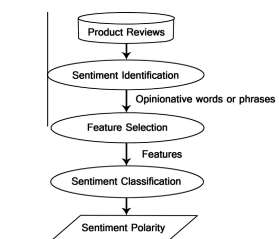
\includegraphics[height=5cm]{text/img/SAProcess.PNG}
    \caption{\todo{Přeložit do češtiny a popisek.}}
    \label{fig:SAprocess}
\end{figure}

Tyto přístupy můžeme rozdělit na dvě základní skupiny: strojové učení a přístup založený na slovníku.

\subsection{Přístupy strojového učení}

Strojové učení se běžně rozděluje na tyto skupiny: \cite{ml1} 

\begin{description}
	\item[Supervizované učení] - Máme k dispozici vstupní data (příznaky) a k nim přiřazený správný výstup (ten může být diskrétní resp. spojitý a potom úlohu nazýváme klasifikační resp. regresní). Díky označeným datům, můžeme trénovat náš model, na základě chyb od originálního výstupu. Data se zde rozdělují do 3 skupin: trénovací, validační, testovací v určitém poměru (zde se zdroje neschodují na stejných hodnotách, většinou se ale jedná o poměr 3:1:1 viz. Obrázek \ref{fig:datasplit}). Trénovací slouží k trénování modelu a jeho parametrů, validační k jeho porovnání s ostatními natrénovanými modely a testovací pak k odhadu chyby našeho modelu. 
	\item[Nesupervizované učení] - Zde nemáme ke vstupním datům odpovídající výstup a autor zde musím sám najít souvislosti. 
	\item[Semi-supervizované učení] - Kombinace supervizovaného a nesupervizovaného učení
	\item[Posilované učení] -  Ayodele jej definuje takto: \uv{Algoritmus se učí pravidla, jak jednat při pozorování světa. Každá akce má nějaký dopad na prostředí a prostředí poskytuje zpětnou vazbu, která řídí algoritmus učení.} \cite[překlad vlastní]{ml1} 
	
	\item[A další] 
\end{description}


\begin{figure}[h]
    \centering
    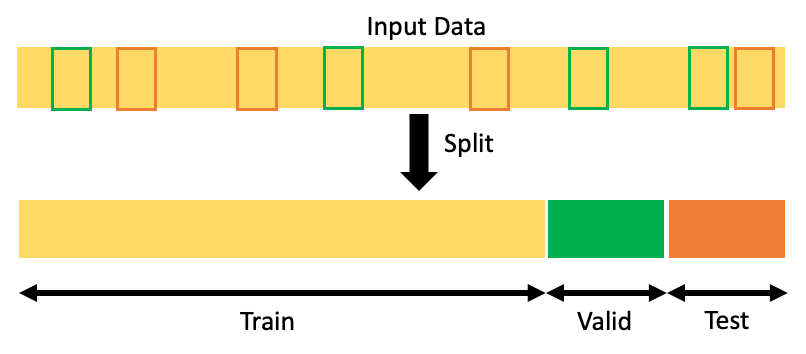
\includegraphics[height=5cm]{text/img/data.png}
    \caption{\todo{Přeložit do češtiny a popisek.}}
    \label{fig:datasplit}
\end{figure}

Medhat ve svém článku ukázal používáné metody z jiných článků zabývajících se analýzou sentimentu. \cite{Medhat} Výčet z kategorie strojového učení pak můžeme vidět na Obrázku \ref{fig:MedhatML}. V následujících kapitolách si tyto metody/modely představíme.

\begin{figure}[h]
    \centering
    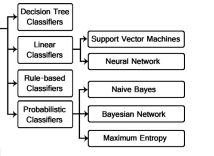
\includegraphics[height=3cm]{text/img/medhatML.PNG}
    \caption{\todo{Přeložit do češtiny a popisek.}}
    \label{fig:MedhatML}
\end{figure}

\subsubsection*{Rozhodovací stromy}
Rozhodovací strom je jednoduchý model, který můžeme použít ke klasifikaci i regresi. Kotsiantis jej definuje takto: \uv{Rozhodovací stromy jsou sekvenční modely, které postupně provádějí jednoduché testy, porovnání;
každý test porovnává číselný atribut s prahovou hodnotou nebo s nominálním atributem
soubor možných hodnot.} \cite[překlad vlastní]{decisionTree} Russel a Norvig jej zase definují obecněji jako \uv{funkci, která jako vstup očekává vektor příznaků a vrací jednu hodnotu -- rozhodnutí}. \cite[překlad vlastní]{aimodern} Oproti jiným modelům jsou rozhodovací stromy také lépe graficky reprezentované (pomocí stromové struktury viz obrázek 
\ref{fig:decisionTree}) a rychlé k pochopení. Výsledek klasifikaci resp. regrese k určitým příznakům zjistíme z daného listu, do kterého se vstupní data postupním porovnáváním listu \textit{dostala}. 



\begin{figure}[h]
    \centering
    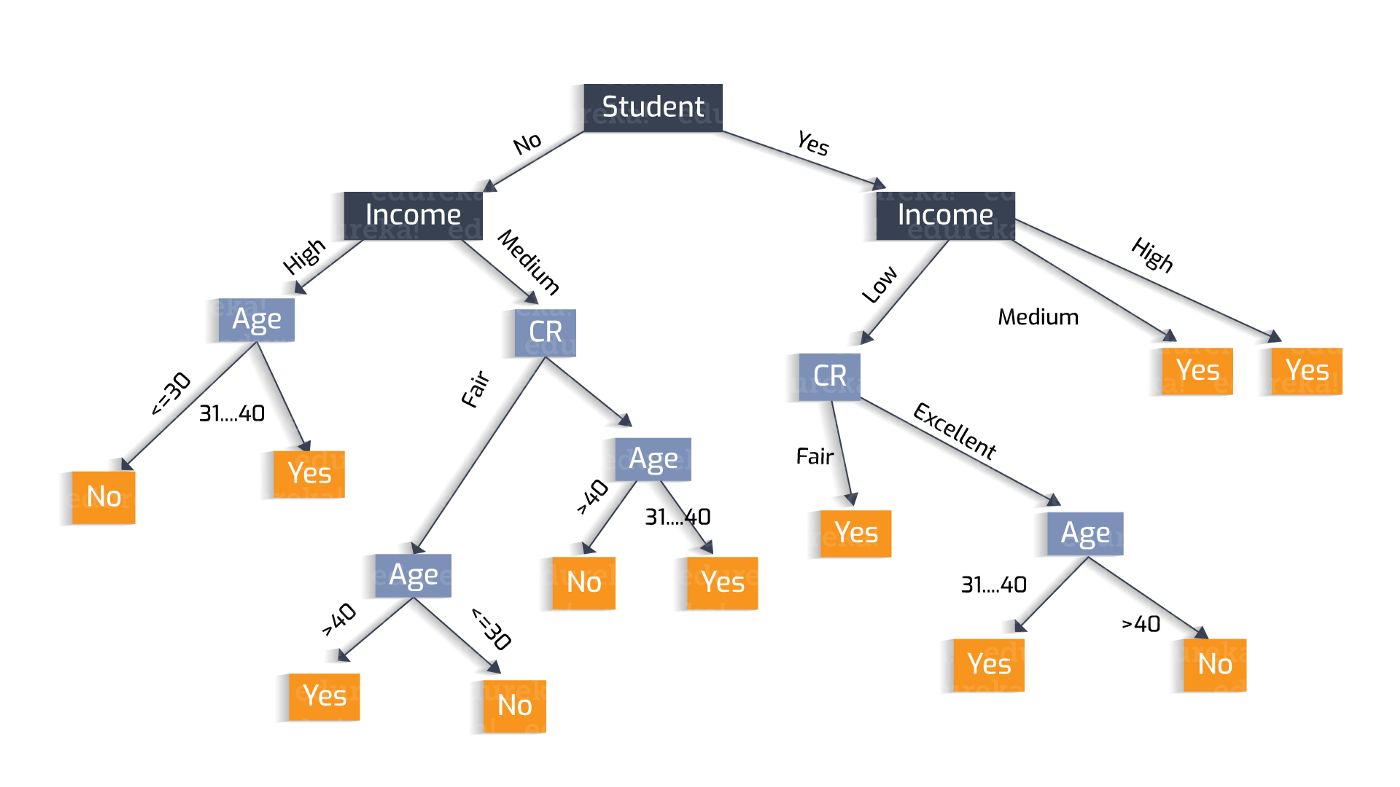
\includegraphics[height=5cm]{text/img/decisionTree.png}
    \caption{\todo{Přeložit do češtiny a popisek.}}
    \label{fig:decisionTree}
\end{figure}

Než vysvětlíme jak stromy vytvářet, budeme k tomu potřebovat různé metriky, pomocí kterých určíme kvalitu rozdělení vektoru příznaků podle určité podmínky.

Jednou z metrik je tzv. \textbf{informační zisk} a vypočítáme ho jako\cite{decisionTrees}:
\[
InformacniZisk(\mathcal{D},X_i) = IG(\mathcal{D}) = H(\mathcal{D}) - \sum^{k-1}_{j = 0} t_j  H(\mathcal{D}_j),
\]kde $\mathcal{D}_j$ je podmnožina $\mathcal{D}$ pro které $X_i = j$, $t_j$ je podíl počtu prvků v $\mathcal{D}_j$ a $\mathcal{D}$. 

Funkce $H(\mathcal{D})$ ve vzorci je pak odhad entropie dat:
\[
Entropie(\mathcal{D}) = H(\mathcal{D}) = - \sum^{k-1}_{i = 0} p_i  \log(p_i),
\]
kde $\mathcal{D}$ je množina dat, $p_i$ je  poměr počtu $i$ v $\mathcal{D}$ a platí $ \sum^{k-1}_{i = 0} p_i = 1$. 


Další metrikou je tzv. \textbf{Gini index}, která udává míru toho, že nově přidaný prvek bude špatně klasifikován. Přesný výpočet je \cite{vzd}:
\[
GiniIndex(\mathcal{D}) = GI(\mathcal{D}) = \sum^{k-1}_{i = 0} p_i  (1 - p_i) 
\]
Gini index můžeme využit při výpočtu informačního zisku, kdy jen ve vzorci nahradíme $(\mathcal{D})$ za  $GI(\mathcal{D})$.

Můžeme

\subsubsection{Naivní Bayesův klasifikátor}
Tento klasifikátor spadá do kategorie pravděbodobnostních klasifikátorů. Klasické klasifikátory jsou reprezentované funkcí, která mapuje vstup (vektor příznaků) na výslednou klasifikační třídu. Narozdíl od nich, pravděbodobnostní klasifikátory vrací podmíněnou pravděbodobnost $p(y|x)$, kde $y$ je výsledná třída  a $x$ je vektor příznaků.

\begin{definition}[Podmíněná pravděbodobnost]
    $$ p(y|x) = \frac{p(y,x)}{p(x)} $$
    \end{definition}

Existují dva přístupy, jak tuto pravděbodobnost dostat. \cite{naiveBayes} \uv{Prvním je přímo vytvořit funkci, která vypočítá určité pravděbodobnosti $p(y|x)$} \cite[překlad vlasntí]{naiveBayes}. Tento model pak nazýváme \textbb{diskriminativní}.

Druhým přístup nazýváme \textbb{generativní}. Pro každou hodnotu $y$ model naučíme $p(x|y)$ a $p(y)$. Poté budeme potřebovat Bayesovu větu \cite{prob}:

    \begin{definition}[Bayesova věta]
        Buďiž $a_1, a_2, \hdots, a_n$ vzájemně disjunktní náhodné jevy, jejichž sjednocení tvoří celý pravděbodobnostní prostor a platí: $\forall i : p(A_i) > 0 $. Pak pro libovný jev $b$ takový, že $p(b) > 0$, platí: 
        $$p(a_i|b) = \frac{p(a_i)p(b|a_i)}{p(b)} = \frac{p(a_i)p(b|a_i)}{\sum_{i=1}^{n}p(b_i|a)p(b_i)}$$
        \end{definition}

Po aplikování Bayesovy věty dostaneme chtěnou pravděbodobnost $p(y|x)$ \cite{naiveBayes}:

$$p(y|x) = \frac{p(x,y)}{p(x)} = \frac{p(x|y)p(y)}{\sum_{y' = 1}^{C}p(x|y')p(y')}$$
Označujeme ho generativním, protože představuje úplnou informaci o rozdělení, ze kterého byla data generována. Výslednou predikci klasifikační třídy pak určíme jako 
$$ Y = arg\,max_y p(y|x)$$

Klasifikátor nazýváme naivním, protože očekává nezávislost všech příznaků:
$$ p(x|y = c) = \prod_{i=1}^{D}p(x_i|y = c)$$
\uv{I přes to, že toto obvykle neplatí (příznaky jsou většinou závislé), výsledný model je jednoduché natrénovat a funguje překvapivě dobře.}\cite[překlad vlastní]{naiveBayes}
\todo{ODHADY PARAMETRŮ}



\appendix\appendixinit % do not remove these two commands

\chapter{Nějaká příloha}


Sem přijde to, co nepatří do hlavní části.
 % include `appendix.tex' from `text/' subdirectory

\backmatter % do not remove this command

\printbibliography % print out the BibLaTeX-generated bibliography list

\chapter{Obsah přiloženého média}


	\dirtree{%
		.1 readme.txt\DTcomment{stručný popis obsahu média}.
		.1 exe\DTcomment{adresář se spustitelnou formou implementace}.
		.1 src.
		.2 impl\DTcomment{zdrojové kódy implementace}.
		.2 thesis\DTcomment{zdrojová forma práce ve formátu \LaTeX{}}.
		.1 text\DTcomment{text práce}.
		.2 thesis.pdf\DTcomment{text práce ve formátu PDF}.
	}
 % include `medium.tex' from `text/' subdirectory

\end{document}
